% A2.2 — Object detection: Faster R-CNN vs DETR on Pascal VOC 2007 + analysis of the DETR paper.
% Compile with XeLaTeX (see latexmkrc).
\documentclass[11pt, a4paper]{article}
\usepackage{bkreport}

\renewcommand{\reporttitleshort}{A2.2 -- Faster R-CNN vs DETR}
\hypersetup{
  pdftitle  = {A2.2\_Faster\_RCNN\_vs\_DETR\_Report\_Hummingbird},
  pdfauthor = {Nguyen Le Hoang Hung, Nguyen Thi Linh Trang}}
\graphicspath{{../../results/}}

\begin{document}
\sloppy   % long \code{...} names may not hyphenate: stretch spaces instead of running into the margin

\makecover{Bài tập lớn A2: Phát hiện đối tượng -- Faster R-CNN vs DETR}
          {Mốc A2.2 -- Cài đặt, so sánh và phân tích paper DETR}
          {TP. Hồ Chí Minh, ngày 16 tháng 11 năm 2026}

\begin{abstract}
Nhóm so sánh Faster R-CNN ResNet-50-FPN (CNN, anchor + NMS) và DETR ResNet-50 (Transformer, dự đoán tập hợp bằng ghép cặp Hungarian) trên Pascal VOC 2007, với cùng dữ liệu, cùng quy tắc resize và cùng cách đánh giá, đồng thời phân tích paper DETR (Carion và cộng sự, ECCV 2020). Khi fine-tune từ checkpoint COCO, DETR đạt mAP@0.5 86,14\% và AP@[.5:.95] 63,0\% trên VOC 2007 test, so với 84,63\% và 56,0\% của Faster R-CNN, và chạy nhanh hơn (28,3 so với 17,5 FPS). Kết quả tái hiện đúng xu hướng của paper: DETR tốt hơn nhiều ở vật lớn (AP$_L$ 71,7 so với 60,8) nhưng kém ở vật nhỏ (AP$_S$ 20,6 so với 26,5). Khi không có pretrain cho bài toán phát hiện (chỉ backbone ImageNet), Faster R-CNN vẫn đạt 76,4\% sau 10 epoch, còn DETR chỉ đạt 2,8\% sau 20 epoch, xác nhận hạn chế lớn nhất của paper là hội tụ chậm. Thí nghiệm theo từng tầng decoder kiểm chứng thêm nhận định rằng DETR không cần NMS.
\end{abstract}

\tableofcontents
\newpage

% =====================================================================
\section{Bài toán và tập dữ liệu}

\subsection{Bài toán}
Phát hiện đối tượng: với mỗi ảnh, dự đoán một tập bounding box, mỗi box kèm một nhãn lớp và một điểm tin cậy. Nhóm so sánh hai cách tiếp cận khác nhau về bản chất: Faster R-CNN~\cite{ren2015faster} với FPN~\cite{lin2017fpn} (CNN, anchor dày đặc, gán nhãn theo IoU, cần NMS) và DETR~\cite{carion2020detr} (Transformer, dự đoán trực tiếp một tập hợp bằng object query, ghép cặp Hungarian, không cần NMS). DETR cũng là paper được phân tích ở Mục~\ref{sec:paper}.

\subsection{Pascal VOC 2007}
Pascal VOC 2007~\cite{everingham2010voc}: 20 lớp; tập trainval 5.011 ảnh, tập test 4.952 ảnh có nhãn đầy đủ. Mỗi đối tượng có box, lớp và cờ \emph{difficult} cho vật khó nhận (bị che khuất nhiều, quá nhỏ). Ảnh lấy từ Flickr, chỉ dùng cho nghiên cứu; repo không chứa ảnh.

\begin{table}[H]
  \centering
  \caption{Split (seed 42). Train/validation lấy ngẫu nhiên từ trainval chính thức; test là tập test chính thức.}
  \label{tab:split}
  \begin{tabular}{lrrrr}
    \toprule
    \textbf{Split} & \textbf{Ảnh} & \textbf{Đối tượng} & \textbf{Difficult} & \textbf{Đối tượng/ảnh (TB / max)} \\
    \midrule
    Train & 4.510 & 14.034 & 2.731 & 3,11 / 42 \\
    Validation & 501 & 1.628 & 323 & 3,25 / 23 \\
    Test & 4.952 & 14.976 & 2.944 & 3,02 / 41 \\
    \bottomrule
  \end{tabular}
\end{table}

\subsection{EDA}
\begin{figure}[H]
  \centering
  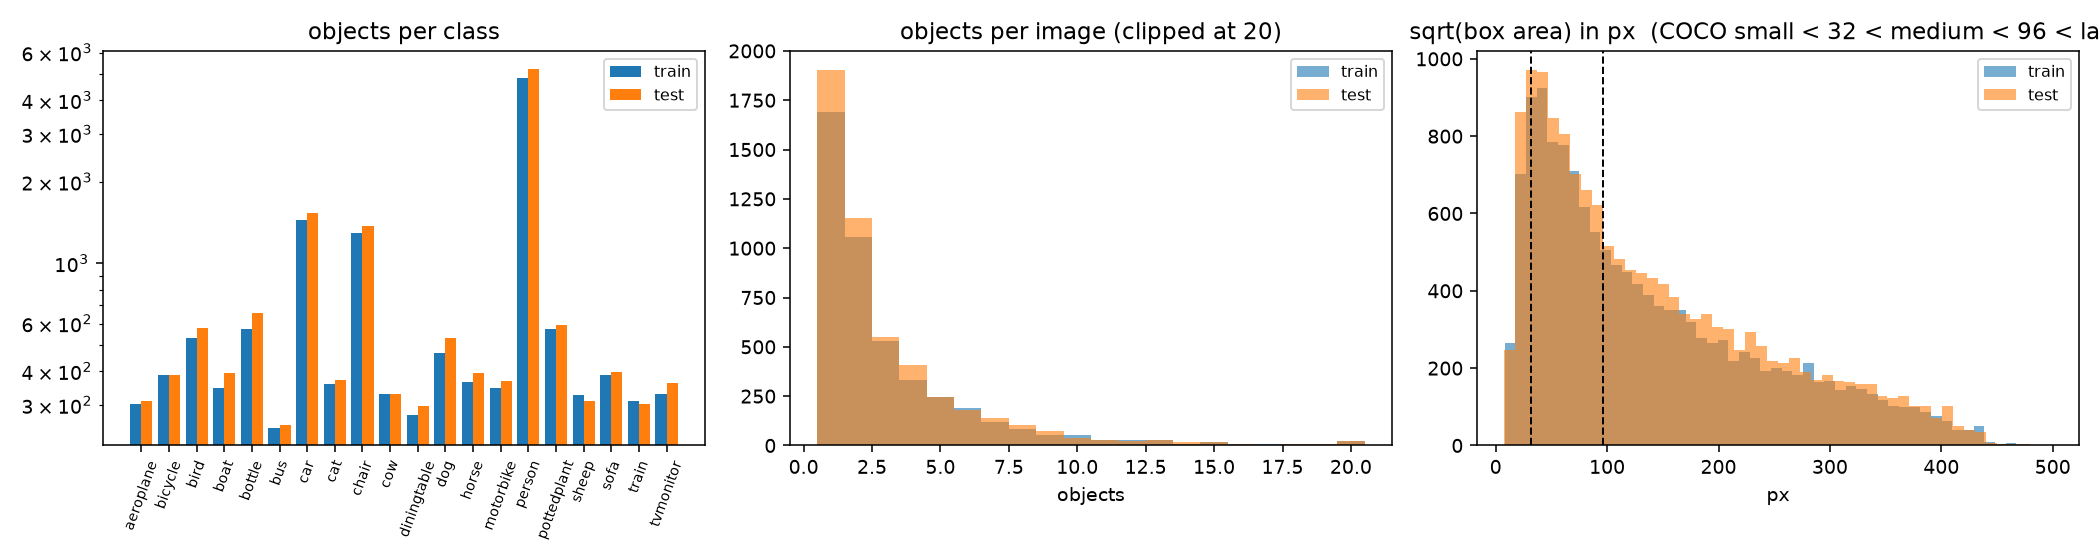
\includegraphics[width=\linewidth]{fig_eda.png}
  \caption{Số đối tượng mỗi lớp (thang log), số đối tượng mỗi ảnh, và căn bậc hai diện tích box với hai ngưỡng nhỏ/vừa/lớn của COCO (32 và 96 px).}
  \label{fig:eda}
\end{figure}

Trung bình khoảng 3 đối tượng mỗi ảnh (tối đa 42), ít hơn hẳn mức 7 của COCO, và luôn nhỏ hơn rất nhiều so với 100 query của DETR. Các lớp lệch mạnh: \emph{person} có 4.823 đối tượng trong tập train, trong khi \emph{bus} chỉ có 248. Khoảng 19\% đối tượng bị đánh dấu difficult. Quan trọng nhất cho việc so sánh với paper: theo ngưỡng của COCO, chỉ 10\% đối tượng test là vật nhỏ, 34\% vật vừa và 55\% vật lớn (COCO có khoảng 41\% vật nhỏ). VOC vì vậy nghiêng về phía vật lớn, là điểm mạnh mà paper báo cáo cho DETR.

% =====================================================================
\section{Dataset, DataLoader và augmentation}

\begin{itemize}
  \item \textbf{Đọc nhãn} (\code{src/voc.py}): phân tích file XML, đổi tọa độ VOC (bắt đầu từ 1) sang hệ bắt đầu từ 0, nhãn 0..19, giữ cờ difficult. Ảnh đọc bằng \code{torchvision.io.read\_image}, trả về tensor $[0,1]$ ở kích thước gốc.
  \item \textbf{Augmentation trên CPU:} lật ngang ngẫu nhiên ($p = 0{,}5$), lật cả box.
  \item \textbf{Resize trên GPU, cùng một quy tắc cho cả hai mô hình} (\code{src/models.py}): khi train, cạnh ngắn chọn ngẫu nhiên trong $\{384, 416, \dots, 608\}$; khi đánh giá, cạnh ngắn 512; cạnh dài tối đa 1000. Paper dùng 480--800 và 1333; nhóm thu nhỏ để vừa GPU 8GB và thời gian. Faster R-CNN dùng \code{GeneralizedRCNNTransform} của torchvision với đúng các tham số này; DETR dùng hàm \code{resize} với cùng công thức.
  \item \textbf{Batch:} 4 ảnh, 6 worker; ảnh kích thước khác nhau nên được giữ dạng danh sách (DETR đệm thành \code{NestedTensor} kèm mask, Faster R-CNN tự gom batch).
  \item \textbf{Đối tượng difficult:} giữ khi train, bỏ qua khi tính mAP (không tính là đúng, không tính là sai), theo quy ước của VOC.
\end{itemize}

% =====================================================================
\section{Phân tích paper DETR}
\label{sec:paper}

\textit{N. Carion, F. Massa, G. Synnaeve, N. Usunier, A. Kirillov, S. Zagoruyko. End-to-End Object Detection with Transformers. ECCV 2020}~\cite{carion2020detr}. Code: \url{https://github.com/facebookresearch/detr}.

\subsection{Ý tưởng}
Các detector trước DETR không dự đoán thẳng ra tập đối tượng. Chúng dự đoán dư thừa trên hàng nghìn anchor hoặc proposal, gán nhãn cho từng anchor bằng luật IoU viết tay, rồi dùng NMS để xóa các box trùng. Kết quả cuối vì vậy phụ thuộc vào nhiều thành phần thủ công. DETR coi phát hiện đối tượng là \textbf{bài toán dự đoán tập hợp}: mô hình xuất ra đúng $N = 100$ dự đoán, và mỗi đối tượng thật phải được giải thích bởi đúng một dự đoán. Hai thành phần làm điều này khả thi là một loss dựa trên ghép cặp một-một, và một Transformer encoder-decoder giải mã song song cả tập.

\subsection{Loss: ghép cặp Hungarian}
Gọi $y = \{y_i\}$ là tập ground truth (được đệm thêm phần tử ``không có vật thể'' $\varnothing$ cho đủ $N$) và $\hat y = \{\hat y_i\}_{i=1}^N$ là tập dự đoán. DETR tìm hoán vị tốt nhất
\begin{equation}
  \hat\sigma = \operatorname*{arg\,min}_{\sigma \in \mathfrak{S}_N} \sum_{i=1}^{N} \mathcal{L}_{\text{match}}(y_i, \hat y_{\sigma(i)}),
\end{equation}
với $\mathcal{L}_{\text{match}} = -\mathbb{1}_{\{c_i \ne \varnothing\}}\,\hat p_{\sigma(i)}(c_i) + \mathbb{1}_{\{c_i \ne \varnothing\}}\,\mathcal{L}_{\text{box}}(b_i, \hat b_{\sigma(i)})$, giải bằng thuật toán Hungarian~\cite{kuhn1955hungarian} (\code{scipy.optimize.linear\_sum\_assignment}). Sau khi ghép, loss là
\begin{equation}
  \begin{split}
  \mathcal{L}_{\text{Hungarian}} = \sum_{i=1}^{N} \Big[ & -\log \hat p_{\hat\sigma(i)}(c_i) \\
    & + \mathbb{1}_{\{c_i \ne \varnothing\}} \big( \lambda_{\text{iou}} \mathcal{L}_{\text{GIoU}}(b_i, \hat b_{\hat\sigma(i)}) + \lambda_{L1} \lVert b_i - \hat b_{\hat\sigma(i)} \rVert_1 \big) \Big],
  \end{split}
\end{equation}
với $\lambda_{L1} = 5$, $\lambda_{\text{iou}} = 2$, trọng số của lớp $\varnothing$ giảm 10 lần để cân bằng, vì phần lớn trong 100 query không ứng với vật thể nào (COCO trung bình 7 vật thể mỗi ảnh, VOC khoảng 3). Box được dự đoán dạng $(c_x, c_y, w, h)$ chuẩn hóa về $[0,1]$. Loss L1 phụ thuộc kích thước box, còn GIoU~\cite{rezatofighi2019giou} thì không, nên hai loss bổ sung cho nhau. Vì mỗi vật thật chỉ được gán cho một dự đoán, các dự đoán trùng bị phạt như ``không có vật thể''. Đây là lý do DETR \emph{không cần NMS}.

Trong code của nhóm: \code{third\_party/detr/models/matcher.py} (chi phí ghép với trọng số 1 / 5 / 2 cho lớp / L1 / GIoU) và \code{SetCriterion} trong \code{models/detr.py}.

\subsection{Kiến trúc}
\begin{enumerate}
  \item \textbf{Backbone:} ResNet-50~\cite{he2016resnet} pretrained ImageNet, BatchNorm đóng băng; ảnh $3 \times H \times W$ cho feature map $2048 \times H/32 \times W/32$.
  \item \textbf{Encoder:} conv $1 \times 1$ giảm xuống $d = 256$ kênh, làm phẳng thành $HW/1024$ token; 6 tầng self-attention + FFN~\cite{vaswani2017attention}. Positional encoding hình sin cố định được cộng vào ở \emph{mọi} tầng attention. Self-attention toàn cục cho phép mỗi vị trí ``nhìn'' toàn ảnh.
  \item \textbf{Decoder:} 6 tầng, nhận $N = 100$ \emph{object query} học được (positional encoding của đầu ra), giải mã \emph{song song} chứ không tự hồi quy. Self-attention giữa các query cho phép chúng ``thương lượng'' để không dự đoán trùng; cross-attention đọc đặc trưng từ encoder.
  \item \textbf{Đầu dự đoán:} một lớp Linear cho lớp (20 + 1 lớp $\varnothing$ trên VOC) và một MLP 3 tầng cho box. \textbf{Auxiliary loss:} cùng một đầu dự đoán (chung tham số) được gắn sau cả 6 tầng decoder, mỗi tầng có loss Hungarian riêng.
\end{enumerate}
Tổng cộng 41,3M tham số, bằng Faster R-CNN-FPN với cùng backbone (42M).

\subsection{Giả thiết ngầm}
(1) Số vật thể mỗi ảnh nhỏ hơn hẳn $N = 100$. (2) Một feature map độ phân giải $1/32$ là đủ, vì attention toàn cục bù được thông tin vị trí. (3) Có đủ dữ liệu và thời gian train để Transformer tự học những gì anchor và NMS mã hóa sẵn. (4) Backbone được pretrain trên ImageNet.

\subsection{Thí nghiệm trong paper}
COCO 2017~\cite{lin2014coco}: 118 nghìn ảnh train, 5 nghìn ảnh val, trung bình 7 vật thể mỗi ảnh (tối đa 63). Metric AP của COCO. AdamW~\cite{loshchilov2019adamw}, lr $10^{-4}$ cho Transformer, $10^{-5}$ cho backbone, weight decay $10^{-4}$, khởi tạo Xavier~\cite{glorot2010xavier}, gradient clipping 0,1. Lịch chuẩn 300 epoch (giảm lr ở epoch 200) mất 3 ngày trên 16 GPU V100 với batch 64; lịch dài 500 epoch cho thêm 1,5 AP.

\begin{table}[H]
  \centering
  \caption{Kết quả chính của paper (Bảng 1, COCO val). Faster R-CNN-FPN+ là bản đã được tăng cường (GIoU, random crop, lịch 9x) để so sánh công bằng.}
  \label{tab:paper}
  \small
  \begin{tabular}{lrrrrrrrr}
    \toprule
    \textbf{Mô hình} & \textbf{GFLOPS/FPS} & \textbf{Tham số} & \textbf{AP} & \textbf{AP50} & \textbf{AP75} & \textbf{AP$_S$} & \textbf{AP$_M$} & \textbf{AP$_L$} \\
    \midrule
    Faster R-CNN-FPN+ & 180 / 26 & 42M & 42,0 & 62,1 & 45,5 & 26,6 & 45,4 & 53,4 \\
    DETR (R50)        & 86 / 28  & 41M & 42,0 & 62,4 & 44,2 & 20,5 & 45,8 & 61,1 \\
    \bottomrule
  \end{tabular}
\end{table}

Kết luận chính của paper: DETR bằng Faster R-CNN đã được tinh chỉnh kỹ về AP tổng, \textbf{tốt hơn nhiều ở vật lớn} (+7,7 AP$_L$) nhưng \textbf{kém ở vật nhỏ} ($-6{,}1$ AP$_S$). Các ablation:
\begin{itemize}
  \item \textbf{Encoder:} bỏ encoder làm AP giảm từ 40,6 xuống 36,7 (giảm 6,0 AP$_L$); attention toàn cục giúp tách các vật thể.
  \item \textbf{Decoder (Hình 4 của paper):} AP tăng sau mỗi tầng, tổng cộng $+8{,}2$ AP giữa tầng đầu và tầng cuối. NMS giúp ích cho dự đoán của tầng đầu (một tầng chưa đủ để các query loại trừ lẫn nhau), nhưng lợi ích giảm dần và ở tầng cuối NMS làm AP giảm nhẹ.
  \item \textbf{FFN:} bỏ FFN (41,3M xuống 28,7M tham số) làm giảm 2,3 AP.
  \item \textbf{Positional encoding:} bỏ hoàn toàn positional encoding không gian làm AP giảm 7,8.
  \item \textbf{Loss:} bỏ GIoU giảm 4,8 AP; bỏ L1 chỉ giảm 0,7 AP.
  \item \textbf{Tổng quát hóa:} tìm được đủ 24 con hươu cao cổ trong một ảnh tổng hợp, trong khi tập train không có ảnh nào quá 13 con.
  \item \textbf{Panoptic segmentation:} thêm một đầu mask, DETR R50 đạt PQ 43,4 so với 42,4 của PanopticFPN++.
\end{itemize}

\subsection{Hạn chế}
\begin{itemize}
  \item \textbf{Chi phí train rất lớn và hội tụ chậm.} 300--500 epoch trên COCO, so với khoảng 36 epoch (lịch 3x) của Faster R-CNN. Nguyên nhân: mỗi vật thật chỉ được gán cho một query, nên tín hiệu giám sát thưa; attention khởi tạo gần như đều trên toàn ảnh và cần rất lâu để học tập trung vào vùng có vật thể; phép ghép Hungarian dao động mạnh ở đầu quá trình train.
  \item \textbf{Yếu ở vật nhỏ.} Chỉ dùng một feature map độ phân giải $1/32$, không có cấu trúc đa tỉ lệ như FPN; tăng độ phân giải (DC5) thì chi phí self-attention tăng theo bình phương số token.
  \item \textbf{Số query cố định} ($N = 100$) giới hạn số vật thể tối đa mỗi ảnh.
  \item \textbf{Phụ thuộc pretrain:} backbone luôn được pretrain ImageNet; paper không thử train từ đầu.
  \item Deformable DETR~\cite{zhu2021deformable} sau đó sửa đúng hai điểm yếu đầu bằng deformable attention đa tỉ lệ, giảm số epoch khoảng 10 lần và cải thiện vật nhỏ.
\end{itemize}

\subsection{Đối chiếu với thí nghiệm của nhóm}
\begin{table}[H]
  \centering
  \caption{Nhận định của paper và kết quả của nhóm trên VOC 2007.}
  \label{tab:compare}
  \small
  \begin{tabularx}{\linewidth}{YYl}
    \toprule
    \textbf{Paper (COCO)} & \textbf{Nhóm (VOC 2007)} & \textbf{Tái hiện?} \\
    \midrule
    DETR ngang Faster R-CNN về AP tổng (42,0 so với 42,0) & DETR hơn: AP 63,0 so với 56,0, mAP@0.5 86,1 so với 84,6 & Một phần \\
    DETR kém ở vật nhỏ (AP$_S$ 20,5 so với 26,6) & AP$_S$ 20,6 so với 26,5 & Có \\
    DETR tốt hơn ở vật lớn (AP$_L$ 61,1 so với 53,4) & AP$_L$ 71,7 so với 60,8 & Có \\
    Cùng cỡ mô hình (41M và 42M), tốc độ tương đương (28 và 26 FPS) & 41,5M và 41,4M; 28,3 và 17,5 FPS & Có (DETR nhanh hơn rõ) \\
    Cần lịch train rất dài & Không có pretrain phát hiện: DETR 2,8\% sau 20 epoch, Faster R-CNN 76,4\% sau 10 epoch & Có \\
    AP tăng qua các tầng decoder (+8,2 AP từ tầng 1 tới 6) & +8,0 AP (55,0 lên 63,0) & Có \\
    NMS giúp tầng đầu, làm giảm nhẹ AP ở tầng cuối & Tầng 1: +2,3 AP; tầng 6: $-0{,}9$ AP & Có \\
    Faster R-CNN cần NMS, DETR thì không & Tắt NMS: Faster R-CNN 84,6 xuống 22,5 mAP@0.5 & Có \\
    \bottomrule
  \end{tabularx}
\end{table}

\paragraph{Những gì nhóm tái hiện được.} Cả ba xu hướng định tính của Bảng 1 (vật nhỏ, vật lớn, chi phí) và hạn chế về hội tụ đều xuất hiện rõ trên VOC, với cùng mã nguồn chính thức của DETR. Ablation theo tầng decoder (Mục~\ref{sec:decoder}) cũng cho con số gần như trùng với paper (+8,0 so với +8,2 AP), và NMS có tác dụng giống paper mô tả: có ích ở tầng đầu, làm giảm nhẹ AP ở tầng cuối.

\paragraph{Những gì khác paper và vì sao.} (1) Trên VOC, DETR \emph{vượt} Faster R-CNN về AP tổng thay vì chỉ ngang bằng: VOC có tỉ lệ vật lớn cao (55\% so với khoảng 24\% của COCO) và trung bình chỉ 3 vật mỗi ảnh, đúng vùng DETR mạnh. (2) Faster R-CNN của nhóm là bản torchvision chuẩn, không có các cải tiến của bản ``FPN+'' trong paper (GIoU, random crop, lịch 9x), và chỉ train 10 epoch. (3) Cả hai được khởi tạo từ checkpoint COCO và fine-tune ngắn, nên kết quả chủ yếu đo khả năng \emph{chuyển giao}, không phải khả năng học từ đầu như paper.

\paragraph{Học được gì cho pipeline.} (1) Muốn dùng DETR trên tập nhỏ thì gần như bắt buộc phải bắt đầu từ checkpoint đã train cho bài toán phát hiện; nếu không, nên chọn Faster R-CNN hoặc biến thể hội tụ nhanh như Deformable DETR. (2) Nếu ứng dụng có nhiều vật nhỏ, cần feature đa tỉ lệ (FPN hoặc deformable attention). (3) Đánh giá bằng AP ở nhiều ngưỡng IoU, không chỉ mAP@0.5, vì lợi thế về độ khít của box chỉ lộ ra ở AP75.

% =====================================================================
\section{Pipeline, huấn luyện và các biến thể}

\subsection{Các biến thể}
\begin{table}[H]
  \centering
  \caption{Các biến thể đã chạy. V4 (DETR không có auxiliary loss) trong kế hoạch A2.1 không chạy vì không đủ thời gian GPU; vai trò của auxiliary head được phân tích bằng thí nghiệm theo từng tầng decoder (Mục~\ref{sec:decoder}).}
  \label{tab:variants}
  \small
  \begin{tabularx}{\linewidth}{llYrr}
    \toprule
    \textbf{Run} & \textbf{Mô hình} & \textbf{Khởi tạo} & \textbf{Epoch} & \textbf{Giảm lr sau} \\
    \midrule
    V1 & Faster R-CNN R50-FPN & checkpoint COCO của torchvision, head mới 21 lớp & 10 & epoch 7 \\
    V2 & DETR R50 & checkpoint COCO chính thức (\code{detr-r50-e632da11.pth}), \code{class\_embed} mới 21 lớp & 20 & epoch 15 \\
    V3 & DETR R50 & chỉ backbone ImageNet; Transformer khởi tạo ngẫu nhiên & 20 & epoch 15 \\
    V5 & Faster R-CNN R50-FPN & chỉ backbone ImageNet; RPN, FPN và head ngẫu nhiên & 10 & epoch 7 \\
    \bottomrule
  \end{tabularx}
\end{table}

\subsection{Cài đặt}
\begin{itemize}
  \item \textbf{Faster R-CNN:} \code{torchvision.models.detection.fasterrcnn\_resnet50\_fpn}, thay \code{box\_predictor} bằng \code{FastRCNNPredictor(1024, 21)}; ngưỡng điểm khi suy luận 0,001, tối đa 100 box mỗi ảnh (để đường PR đầy đủ như DETR, vốn luôn trả về 100 dự đoán).
  \item \textbf{DETR:} dùng nguyên văn \code{models/} và \code{util/} của repo chính thức (\code{A2/third\_party/detr}, giấy phép Apache-2.0), dựng bằng hàm \code{build()} của repo với các tham số mặc định của \code{main.py} (6 + 6 tầng, $d = 256$, 8 head, 100 query, auxiliary loss). Phần nhóm tự viết (\code{src/models.py}): resize/chuẩn hóa, đổi box sang $(c_x, c_y, w, h)$ chuẩn hóa, nạp checkpoint bỏ \code{class\_embed}, và tổng loss theo \code{weight\_dict}.
  \item \textbf{Hai mô hình train cùng phần backbone:} cả hai khóa \code{conv1} và \code{layer1}, dùng FrozenBatchNorm (mặc định của cả hai thư viện), và có số tham số gần như bằng nhau (Bảng~\ref{tab:results}).
  \item \textbf{Training loop chung} (\code{src/train.py}): forward $\rightarrow$ loss $\rightarrow$ \code{backward()} $\rightarrow$ \code{optimizer.step()}. Sau mỗi epoch đo mAP@0.5 trên validation; checkpoint tốt nhất được đánh giá một lần trên test.
\end{itemize}

\begin{table}[H]
  \centering
  \caption{Optimizer. Faster R-CNN theo công thức tham chiếu của torchvision (SGD); DETR theo paper.}
  \label{tab:optim}
  \small
  \begin{tabular}{lll}
    \toprule
    & \textbf{Faster R-CNN (V1, V5)} & \textbf{DETR (V2, V3)} \\
    \midrule
    Optimizer & SGD, momentum 0,9 & AdamW \\
    Learning rate & 0,01 (warm-up tuyến tính 500 bước) & $10^{-4}$ Transformer, $10^{-5}$ backbone \\
    Weight decay & $10^{-4}$ & $10^{-4}$ \\
    Gradient clipping & -- & max norm 0,1 \\
    Lịch lr & chia 10 sau epoch 7 & chia 10 sau epoch 15 \\
    Batch & 4 & 4 \\
    \bottomrule
  \end{tabular}
\end{table}

\paragraph{Độ chính xác số.} Đo trên GTX 1070 (Pascal, không có Tensor Core), autocast fp16 lại \emph{chậm hơn} fp32 với cả hai mô hình (Faster R-CNN 0,83 so với 0,71 giây mỗi bước; DETR 0,60 so với 0,53 giây), nên mọi run dùng fp32.

\paragraph{Metric} (\code{src/evaluate.py}). mAP@0.5 theo VOC, tự cài đặt: đối tượng difficult bị bỏ qua, báo cáo cả diện tích dưới đường PR (VOC2010+) và nội suy 11 điểm (VOC2007). AP@[.5:.95], AP75, AP$_S$/AP$_M$/AP$_L$ theo COCO bằng \code{pycocotools}, với đối tượng difficult được đánh dấu là vùng ``crowd'' để bị bỏ qua. Cả hai cách tính được kiểm tra bằng cách đưa chính ground truth làm dự đoán: đều cho 100\%. FPS đo ở batch 1, độ phân giải test, gồm cả resize và hậu xử lý.

\subsection{Thay đổi so với kế hoạch A2.1}
\begin{itemize}
  \item Số epoch giảm từ 12 xuống 10 (Faster R-CNN) và từ 25 xuống 20 (DETR) để tổng thời gian train vừa với khoảng 11 giờ GPU còn lại; đo thực tế một epoch mất khoảng 13 phút (Faster R-CNN) và 10 phút (DETR).
  \item Không dùng random crop (đã ghi là tùy chọn trong A2.1); không chạy V4.
  \item fp32 thay cho AMP (đo ở trên).
\end{itemize}

% =====================================================================
\section{Kết quả}

\subsection{Bảng tổng hợp}

\begin{table}[H]
  \centering
  \caption{Kết quả trên VOC 2007 test (4.952 ảnh) với checkpoint có mAP@0.5 validation cao nhất. mAP@0.5: diện tích dưới đường PR (VOC2010+); 11-pt: nội suy 11 điểm (VOC2007). AP, AP75, AP$_S$/AP$_M$/AP$_L$ theo COCO. Thời gian train trên GTX 1070; FPS ở batch 1, cạnh ngắn 512.}
  \label{tab:results}
  \footnotesize
  \setlength{\tabcolsep}{3pt}
  \begin{tabular}{lrrrrrrrrrrr}
    \toprule
    \textbf{Run} & \textbf{Tham số} & \textbf{Epoch} & \textbf{mAP@0.5} & \textbf{11-pt} & \textbf{AP} & \textbf{AP75} & \textbf{AP$_S$} & \textbf{AP$_M$} & \textbf{AP$_L$} & \textbf{Giờ train} & \textbf{FPS} \\
    \midrule
    V1 Faster R-CNN (COCO) & 41,4M & 10 & \textbf{84,6} & 81,3 & 56,0 & 62,5 & 26,5 & 42,5 & 60,8 & 2,12 & 17,5 \\
    V2 DETR (COCO) & 41,5M & 20 & \textbf{86,1} & 83,0 & 63,0 & 68,8 & 20,6 & 42,2 & 71,7 & 2,81 & 28,3 \\
    V5 Faster R-CNN (ImageNet) & 41,4M & 10 & \textbf{76,4} & 74,1 & 42,9 & 43,8 & 16,5 & 30,9 & 47,0 & 1,87 & 17,5 \\
    V3 DETR (ImageNet) & 41,5M & 20 & \textbf{2,8} & 5,1 & 1,0 & 0,5 & 0,0 & 0,1 & 1,4 & 2,82 & 28,2 \\
    \bottomrule
  \end{tabular}
\end{table}

\begin{figure}[H]
  \centering
  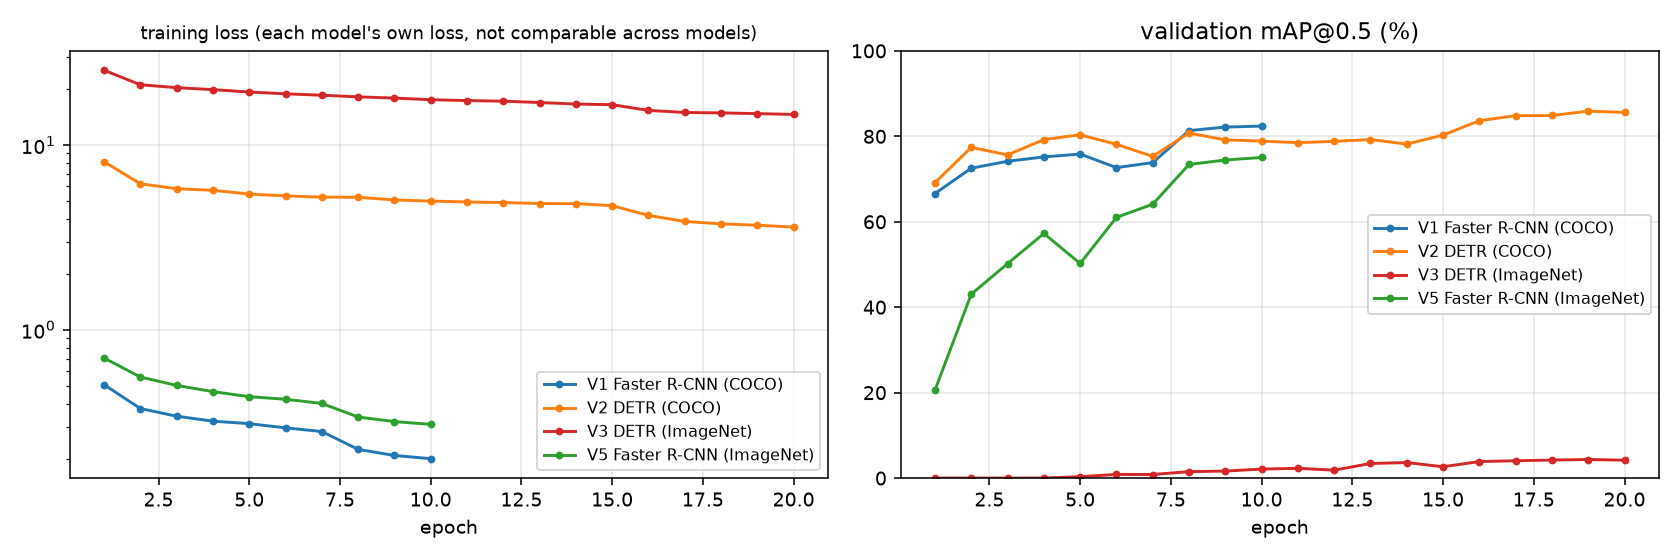
\includegraphics[width=\linewidth]{fig_curves.png}
  \caption{Loss train (thang log; mỗi mô hình có loss riêng nên chỉ so được hình dạng) và mAP@0.5 validation theo epoch. Các bước nhảy ở epoch 8 (Faster R-CNN) và 16 (DETR) là lúc learning rate giảm 10 lần.}
  \label{fig:curves}
\end{figure}

\subsection{Theo kích thước vật thể và theo lớp}

\begin{figure}[H]
  \centering
  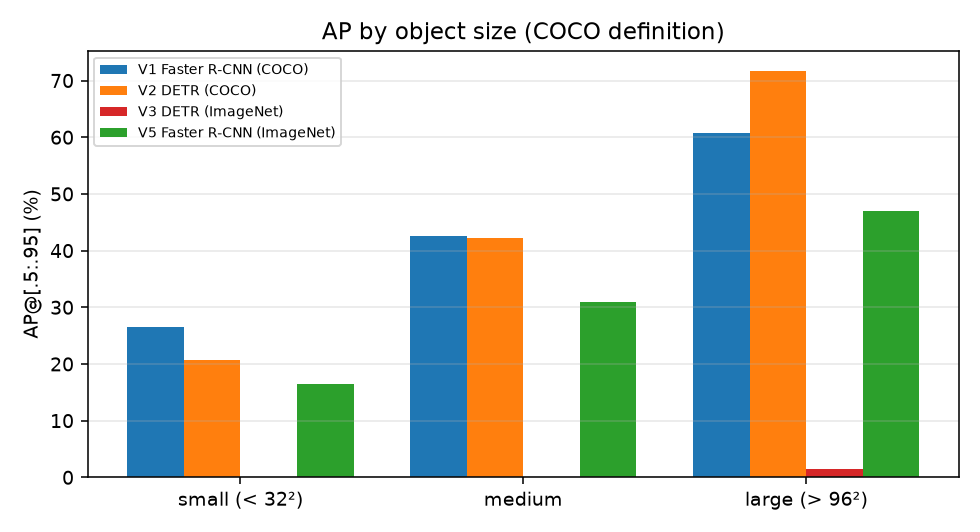
\includegraphics[width=0.75\linewidth]{fig_ap_by_size.png}
  \caption{AP@[.5:.95] theo kích thước vật thể (định nghĩa của COCO).}
  \label{fig:sizes}
\end{figure}

\begin{figure}[H]
  \centering
  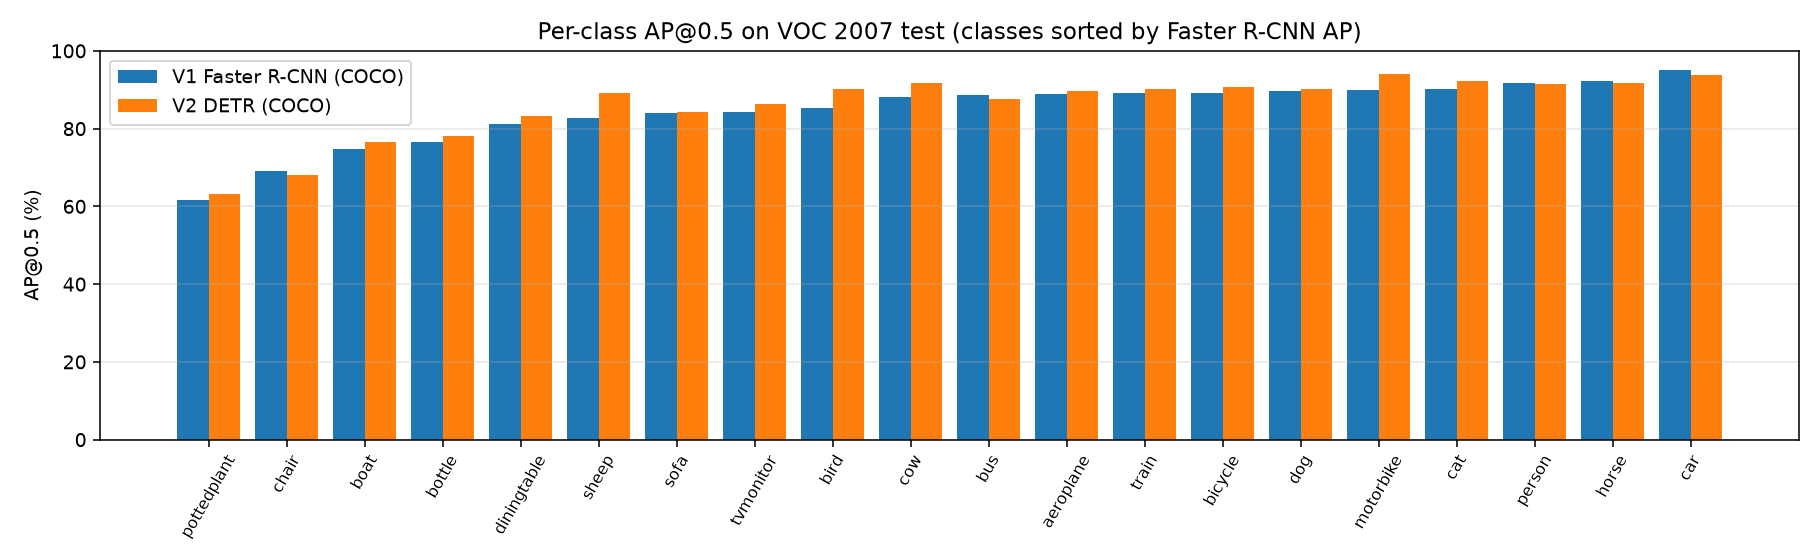
\includegraphics[width=\linewidth]{fig_per_class.png}
  \caption{AP@0.5 theo lớp của V1 và V2, sắp xếp theo AP của Faster R-CNN.}
  \label{fig:perclass}
\end{figure}

\begin{figure}[H]
  \centering
  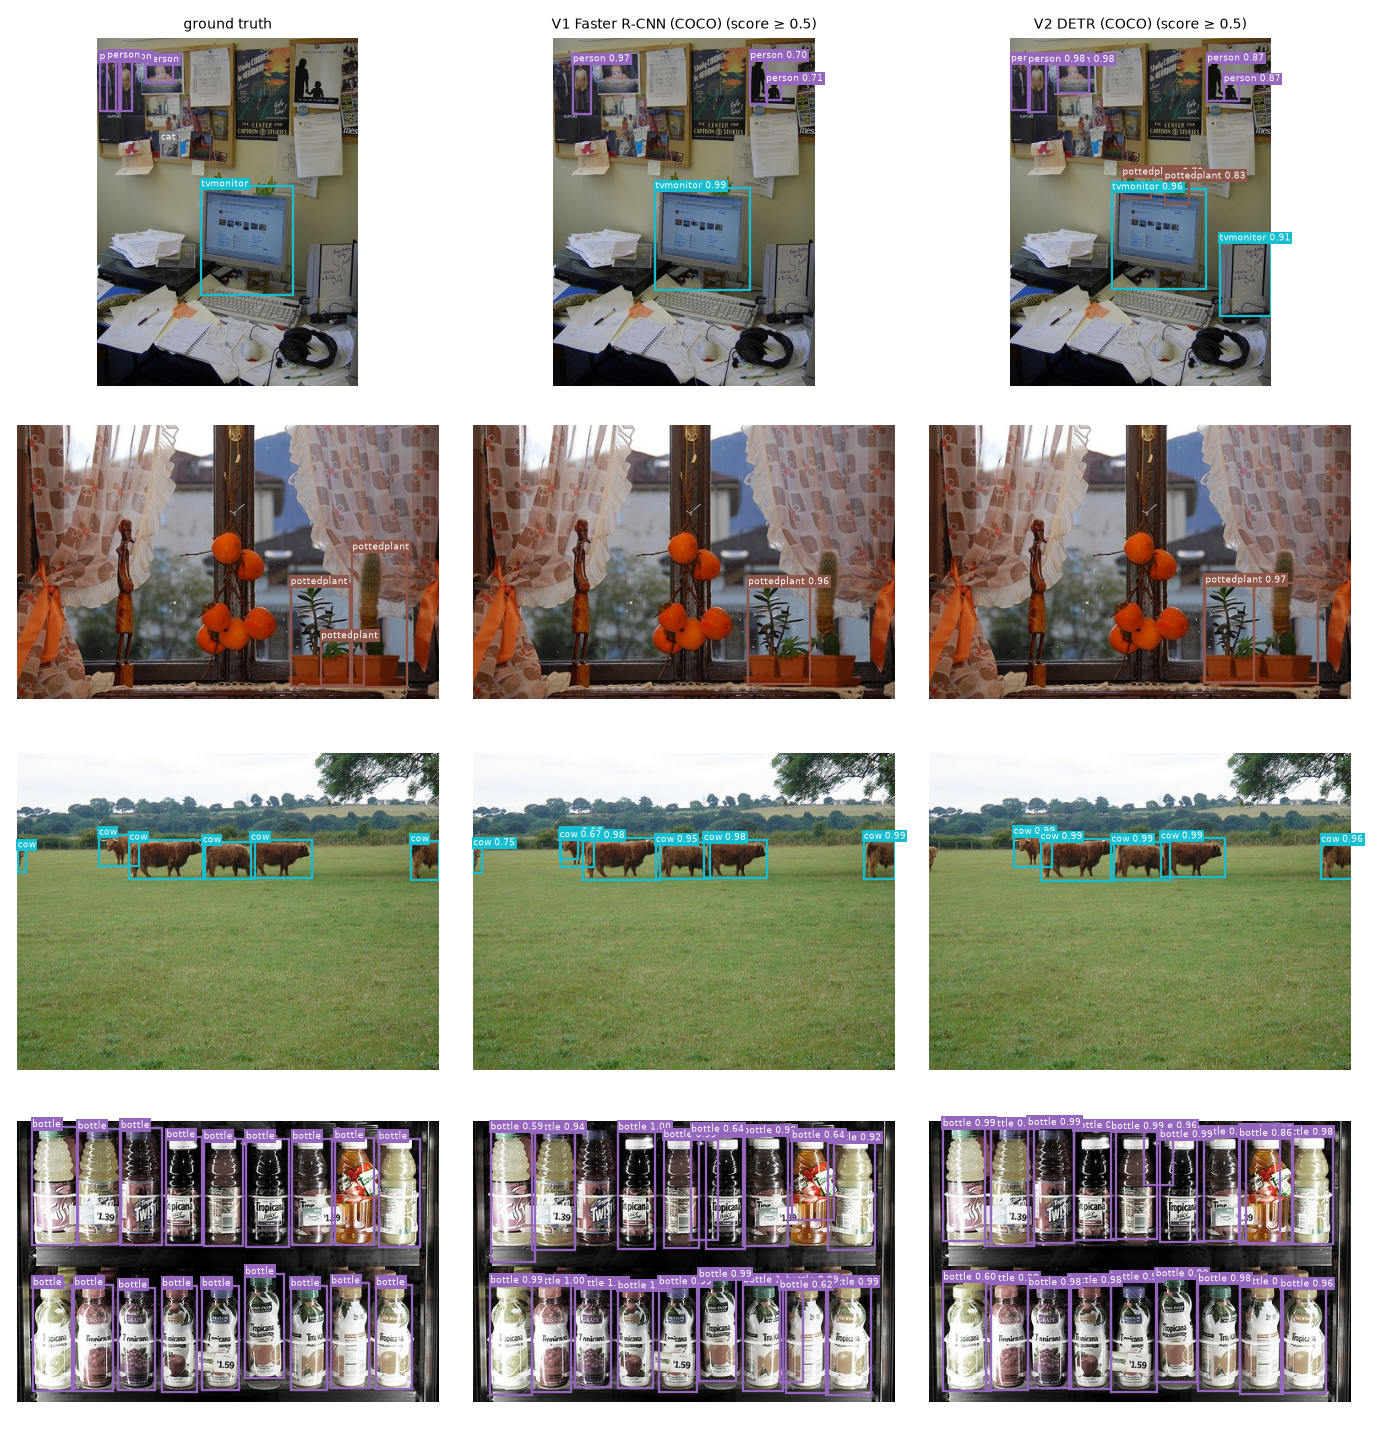
\includegraphics[width=\linewidth]{fig_examples.png}
  \caption{Cùng bốn ảnh test: ground truth, dự đoán của Faster R-CNN và của DETR (điểm $\ge 0{,}5$).}
  \label{fig:examples}
\end{figure}

\subsection{Kiểm chứng hai nhận định của paper (chỉ đánh giá, không train thêm)}
\label{sec:decoder}
Mục này dùng lại các checkpoint đã train, không train thêm. Với DETR, nhờ auxiliary head, một lần forward cho ra dự đoán sau cả 6 tầng decoder; mỗi tầng được đánh giá có và không có NMS (\texttt{batched\_nms}, IoU 0,5, theo từng lớp), như Hình~4 của paper. Với Faster R-CNN, nhóm tắt NMS bằng cách đặt ngưỡng NMS của ROI head bằng 1,0.

\begin{figure}[H]
  \centering
  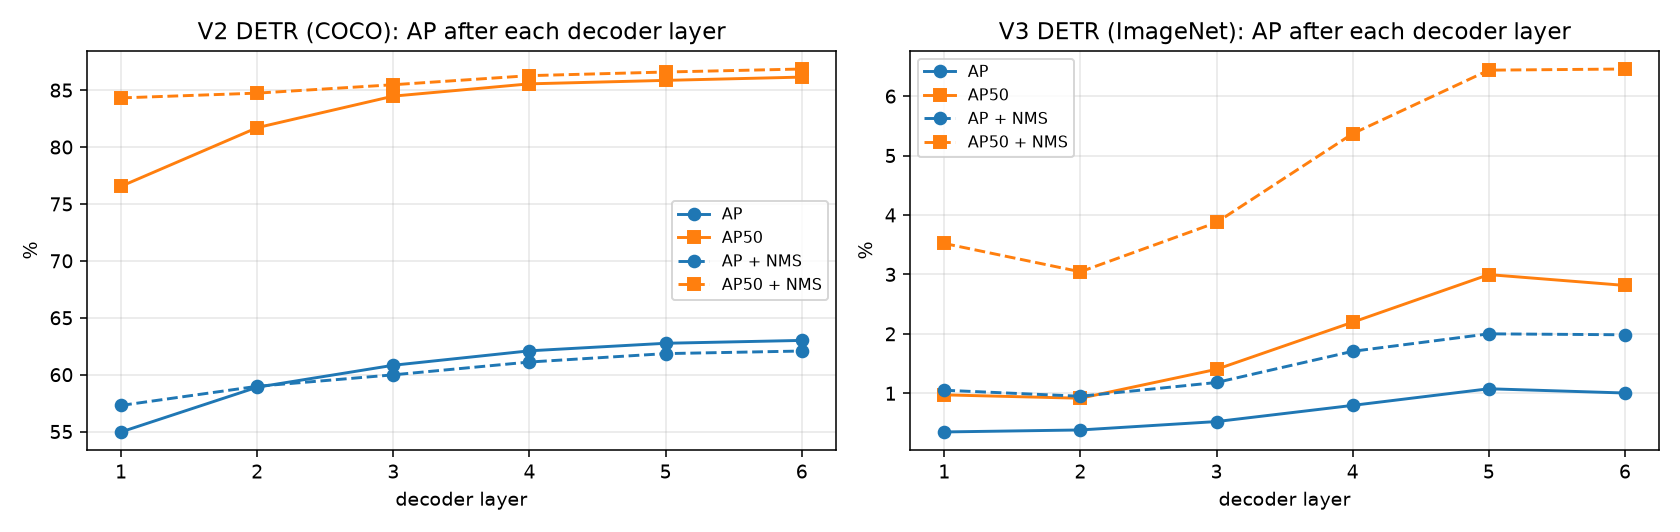
\includegraphics[width=\linewidth]{fig_decoder_layers.png}
  \caption{AP@[.5:.95] và AP@0.5 sau từng tầng decoder, có (nét đứt) và không có NMS. Trái: V2; phải: V3 (lưu ý thang trục tung khác nhau).}
  \label{fig:decoder}
\end{figure}

\begin{table}[H]
  \centering
  \caption{AP theo tầng decoder của V2 (DETR, COCO) trên VOC 2007 test (\%).}
  \label{tab:decoder}
  \small
  \begin{tabular}{crrrrrr}
    \toprule
    & \multicolumn{3}{c}{\textbf{Không NMS}} & \multicolumn{3}{c}{\textbf{Có NMS}} \\
    \cmidrule(lr){2-4}\cmidrule(lr){5-7}
    \textbf{Tầng} & AP & AP$_{50}$ & AP$_S$ & AP & AP$_{50}$ & AP$_S$ \\
    \midrule
    1 & 55,0 & 76,6 & 13,2 & 57,3 & 84,3 & 15,1 \\
    2 & 58,9 & 81,7 & 17,2 & 59,0 & 84,7 & 17,8 \\
    3 & 60,8 & 84,5 & 18,9 & 60,0 & 85,5 & 18,6 \\
    4 & 62,1 & 85,6 & 20,1 & 61,1 & 86,3 & 19,8 \\
    5 & 62,8 & 85,9 & 20,7 & 61,8 & 86,6 & 20,6 \\
    6 & \textbf{63,0} & 86,1 & 20,6 & 62,1 & \textbf{86,9} & 20,4 \\
    \bottomrule
  \end{tabular}
\end{table}

\paragraph{Chất lượng tăng dần qua các tầng decoder.} Không dùng NMS, AP của V2 tăng từ 55,0 ở tầng 1 lên 63,0 ở tầng 6 (+8,0 điểm). Paper báo +8,2 AP trên COCO, nên con số gần như trùng khớp. Phần lớn mức tăng nằm ở ba tầng đầu (+5,8); ba tầng sau chỉ thêm 2,2 điểm. AP$_S$ tăng từ 13,2 lên 20,6, nhưng vẫn kém xa 26,5 của Faster R-CNN: nhiều tầng decoder không bù được việc thiếu feature độ phân giải cao.

\paragraph{NMS chỉ có ích ở các tầng đầu.} Ở tầng 1, NMS tăng AP thêm 2,3 điểm và AP$_{50}$ thêm 7,7 điểm: các query chưa trao đổi thông tin đủ nhiều qua self-attention nên vẫn sinh ra dự đoán trùng cho cùng một vật. Từ tầng 3 trở đi, NMS \emph{làm giảm} AP (tầng 6: 63,0 xuống 62,1), vì nó xóa nhầm một số dự đoán đúng của các vật nằm sát nhau. Đây đúng là xu hướng paper mô tả: NMS cải thiện tầng đầu, còn ở tầng cuối gây mất một ít AP. Một chi tiết khác paper: ở tầng 6, AP$_{50}$ vẫn tăng nhẹ khi có NMS (86,1 lên 86,9), nghĩa là vẫn còn ít box trùng ở ngưỡng IoU lỏng, nhưng cái giá ở các ngưỡng IoU chặt lớn hơn phần lợi này.

\paragraph{DETR chưa hội tụ (V3) vẫn cần NMS.} Với V3, NMS tăng AP$_{50}$ ở tầng 6 từ 2,8 lên 6,5 (gấp hơn hai lần). Như vậy khả năng ``tự khử trùng lặp'' không phải là thuộc tính có sẵn của kiến trúc mà là thứ DETR phải \emph{học được} qua loss ghép cặp một-một; sau 20 epoch không có pretrain, mô hình chưa học được điều đó.

\paragraph{Faster R-CNN không thể bỏ NMS.} Khi tắt NMS, mAP@0.5 của V1 giảm từ 84,6 xuống 22,5 và AP@[.5:.95] từ 56,0 xuống 17,5. Mỗi vật được nhiều anchor và proposal cùng dự đoán, nên không có NMS sẽ có rất nhiều box trùng, và tất cả trừ một box đều bị tính là dự đoán sai. Điều này xác nhận luận điểm trung tâm của paper: NMS là thành phần bắt buộc của Faster R-CNN, còn DETR đã thay nó bằng loss ghép cặp.


% =====================================================================
\section{Thảo luận}

\subsection{CNN và Transformer khi có pretrain COCO (V1 và V2)}
DETR hơn Faster R-CNN 1,5 điểm mAP@0.5 nhưng hơn tới 7,0 điểm AP@[.5:.95] và 6,3 điểm AP75: khoảng cách lớn dần khi ngưỡng IoU chặt hơn, nghĩa là box của DETR khít với vật hơn. Loss GIoU (không phụ thuộc kích thước) và việc mỗi vật chỉ được gán một dự đoán giải thích được điều này. Theo lớp, DETR thắng ở 15/20 lớp; lợi thế lớn nhất ở sheep (+6,5), bird (+4,9) và motorbike (+4,1). Một giả thuyết hợp lý là sheep, bird và cow thường xuất hiện thành đàn với nhiều con chồng lên nhau, nơi suy luận toàn cục và việc mỗi query chỉ nhận một vật giúp tách từng con; nhóm chưa kiểm chứng riêng điều này. Faster R-CNN chỉ hơn ở car, bus, chair, horse, person, mỗi lớp không quá 1,1 điểm.

\subsection{Vật nhỏ và vật lớn}
DETR kém Faster R-CNN 5,9 điểm ở vật nhỏ, ngang nhau ở vật vừa và hơn 10,8 điểm ở vật lớn. Trong Hình~\ref{fig:examples} (hàng thứ ba), Faster R-CNN phát hiện con bò nhỏ ở xa bên trái còn DETR bỏ sót. Nguyên nhân là DETR chỉ nhìn feature map độ phân giải $1/32$, trong khi FPN của Faster R-CNN có thêm các tầng $1/4$ đến $1/16$. Vì VOC có tới 55\% vật lớn và chỉ 10\% vật nhỏ, điểm yếu này ảnh hưởng ít tới mAP tổng; trên COCO (41\% vật nhỏ), paper chỉ thấy hai mô hình ngang nhau.

\subsection{Hội tụ: khi không có pretrain cho bài toán phát hiện (V3 và V5)}
Đây là khác biệt lớn nhất trong thí nghiệm. Faster R-CNN chỉ có backbone ImageNet (V5) đạt 20,6\% mAP@0.5 validation sau 1 epoch và 76,4\% trên test sau 10 epoch. DETR trong cùng điều kiện (V3) có mAP gần 0 trong 4 epoch đầu và chỉ đạt 4,4\% validation (2,8\% test) sau 20 epoch, dù loss vẫn giảm đều. Faster R-CNN mã hóa sẵn kiến thức về vị trí và kích thước qua anchor, và mỗi vật được gán cho nhiều anchor, nên có rất nhiều tín hiệu giám sát ngay từ đầu. DETR phải tự học cả việc ``nhìn vào đâu'' (attention ban đầu gần như đều trên toàn ảnh) lẫn cách phân công 100 query, với chỉ một dự đoán được giám sát cho mỗi vật. Đây chính là lý do paper cần 300--500 epoch trên COCO; trên VOC với 20 epoch, Transformer của DETR mới ở giai đoạn đầu.

\subsection{Chi phí}
Hai mô hình có số tham số gần như bằng nhau (41,4M và 41,5M, như Bảng 1 của paper). Một epoch DETR nhanh hơn (8.4 so với 12.7 phút) vì không có RPN, RoIAlign và lấy mẫu proposal, nhưng DETR cần gấp đôi số epoch nên tổng thời gian dài hơn (2,81 so với 2,12 giờ). Khi suy luận, DETR nhanh hơn 1,6 lần (28,3 so với 17,5 FPS) vì không có NMS và chỉ xử lý 100 query; paper đo 28 so với 26 FPS trên V100 ở độ phân giải lớn hơn.

\subsection{Hạn chế của thí nghiệm}
\begin{itemize}
  \item Lịch train ngắn so với paper (20 so với 300--500 epoch cho DETR); V3 chắc chắn chưa hội tụ.
  \item Một seed duy nhất; không có khoảng tin cậy. Với gần 5.000 ảnh test, chênh lệch dưới khoảng 1 điểm mAP nên được coi là không đáng kể.
  \item Độ phân giải thấp hơn paper (cạnh ngắn 512 khi test so với 800), làm vật nhỏ khó hơn cho cả hai mô hình.
  \item Không tinh chỉnh hyperparameter; Faster R-CNN dùng lr 0,01 cho batch 4, cao hơn mức tuyến tính theo công thức tham chiếu (0,005).
\end{itemize}

% =====================================================================
\section{Kết luận}
Trên Pascal VOC 2007 và một GTX 1070, DETR fine-tune từ COCO đạt mAP@0.5 86,14\% và AP 63,0\%, vượt Faster R-CNN (84,63\% và 56,0\%) và nhanh hơn khi suy luận. Kết quả tái hiện các nhận định chính của paper: DETR tốt hơn ở vật lớn, kém ở vật nhỏ, không cần NMS, và hội tụ rất chậm khi Transformer phải học từ đầu (2,8\% so với 76,4\% của Faster R-CNN cùng điều kiện). Với tập dữ liệu nhỏ, lợi thế của DETR chỉ dùng được khi có checkpoint đã train cho bài toán phát hiện.

\section*{Tái lập kết quả}
\addcontentsline{toc}{section}{Tái lập kết quả}
Code: \url{https://github.com/hwnghoang/cs_deeplearning/tree/main/A2}. Từ thư mục \code{A2/}: \code{python run\_all.py} (4 run, log và kết quả trong \code{results/}), \code{python -m src.ablate} (thí nghiệm theo tầng decoder và NMS), \code{python -m src.analyze} (bảng và hình). Tải dữ liệu, checkpoint và môi trường: \code{A2/README.md}.

\bibliographystyle{plainnat}
\bibliography{refs}

\end{document}
